\begin{enumerate}[label=\thesubsection.\arabic*, ref=\thesubsection.\theenumi]
\item A tangent to a circle with centre $\vec{O}$ is perpendicular to the radius through the point of contact $\vec{T}$,
\begin{align}
	\brak{\vec{P}-\vec{T}}^{\top}\brak{\vec{T}-\vec{O}} = 0
	\label{eq:EE26BTECH11229-tangent-perp}
\end{align}
where $\vec{P}$ is any other point on the tangent.
\item The lengths of the two tangents drawn from an external point $\vec{P}$ to a circle of radius $a$ and centre $\vec{O}$ are equal and
\begin{align}
	\norm{\vec{P}-\vec{T}_1} = \norm{\vec{P}-\vec{T}_2} = \sqrt{\norm{\vec{P}-\vec{O}}^2 - a^2}
	\label{eq:EE26BTECH11229-tangent-equal}
\end{align}
where $\vec{T}_1$ and $\vec{T}_2$ are the points of contact.
\\
\solution
From \eqref{eq:EE26BTECH11229-tangent-perp} and Pythagoras' theorem in the right triangle $\vec{O}\vec{T}_i\vec{P}$, $i=1,2$,
\begin{align}
	\norm{\vec{P}-\vec{O}}^2 = \norm{\vec{P}-\vec{T}_i}^2 + \norm{\vec{T}_i-\vec{O}}^2
	= \norm{\vec{P}-\vec{T}_i}^2 + a^2
\end{align}
which is the same for $i=1,2$, yielding \eqref{eq:EE26BTECH11229-tangent-equal}.
\item In a right triangle with an acute angle $\theta$,
\begin{align}
	\sin\theta = \frac{\text{opposite}}{\text{hypotenuse}}, \quad
	\tan\theta = \frac{\text{opposite}}{\text{adjacent}}
	\label{eq:EE26BTECH11229-trig}
\end{align}
\item The angle $\theta$ between the vectors $\vec{a}$ and $\vec{b}$ is given by
\begin{align}
	\cos\theta = \frac{\vec{a}^{\top}\vec{b}}{\norm{\vec{a}}\norm{\vec{b}}}
	\label{eq:EE26BTECH11229-angle-vec}
\end{align}
For complementary angles,
\begin{align}
	\cos\brak{90^{\circ}-\theta} = \sin\theta, \quad \cos^2\theta + \cos^2\brak{90^{\circ}-\theta} = 1
\end{align}
\item The locus of a point $\vec{x}$ equidistant from the points $\vec{A}$ and $\vec{B}$ is
\begin{align}
	\brak{\vec{A}-\vec{B}}^{\top}\vec{x} = \frac{\norm{\vec{A}}^2 - \norm{\vec{B}}^2}{2}
	\label{eq:EE26BTECH11229-perp-bisector}
\end{align}
\solution
\begin{align}
	\norm{\vec{x}-\vec{A}}^2 &= \norm{\vec{x}-\vec{B}}^2
	\\
	\implies \norm{\vec{x}}^2 - 2\vec{A}^{\top}\vec{x} + \norm{\vec{A}}^2
	&= \norm{\vec{x}}^2 - 2\vec{B}^{\top}\vec{x} + \norm{\vec{B}}^2
\end{align}
which simplifies to \eqref{eq:EE26BTECH11229-perp-bisector}.
\item For the quadratic equation $px^2 + qx + r = 0$ with roots $\alpha$ and $\beta$,
\begin{align}
	\alpha + \beta = -\frac{q}{p}, \quad \alpha\beta = \frac{r}{p}
	\label{eq:EE26BTECH11229-quad-roots}
\end{align}
\item The $n^{\text{th}}$ term of an A.P. with first term $a$ and common difference $d$ is
\begin{align}
	a_n = a + \brak{n-1}d
	\label{eq:EE26BTECH11229-ap-nth}
\end{align}
\item If $\vec{R}$ lies on the line through $\vec{P}$ and $\vec{Q}$, then
\begin{align}
	\vec{R} - \vec{P} = \lambda\brak{\vec{Q} - \vec{P}}
	\label{eq:EE26BTECH11229-ratio-collinear}
\end{align}
for some scalar $\lambda$, and $\vec{R}$ divides the line segment $\vec{P}\vec{Q}$ in the ratio
\begin{align}
	\vec{P}\vec{R} : \vec{R}\vec{Q} = \lambda : \brak{1 - \lambda}
\end{align}
\solution
From \eqref{eq:EE26BTECH11229-collinear}, the columns of $\myvec{\vec{Q}-\vec{P} & \vec{R}-\vec{P}}$ are linearly dependent, which gives the first equation. Then
\begin{align}
	\vec{R} - \vec{Q} = \brak{\lambda - 1}\brak{\vec{Q} - \vec{P}}
\end{align}
so $\norm{\vec{R}-\vec{P}} : \norm{\vec{R}-\vec{Q}} = \abs{\lambda} : \abs{1-\lambda}$, yielding the ratio.
\item The points $\vec{A}$, $\vec{B}$ and $\vec{C}$ are collinear if and only if
\begin{align}
	\rank\myvec{\vec{B}-\vec{A} & \vec{C}-\vec{A}} = 1
	\label{eq:EE26BTECH11229-collinear}
\end{align}
\item The roots of the quadratic equation $px^2 + qx + r = 0$ are
\begin{align}
	x = \frac{-q \pm \sqrt{q^2 - 4pr}}{2p}
	\label{eq:EE26BTECH11229-quad-formula}
\end{align}
The roots are equal if and only if
\begin{align}
	q^2 - 4pr = 0
	\label{eq:EE26BTECH11229-quad-equal}
\end{align}
\item The equation of a conic is
\begin{align}
	\vec{x}^{\top}\vec{V}\vec{x} + 2\vec{u}^{\top}\vec{x} + f = 0
	\label{eq:EE26BTECH11229-conic}
\end{align}
where $\vec{V}$ is a symmetric matrix. It is a parabola if $\rank\brak{\vec{V}} = 1$. The points of intersection with the line $\vec{x} = \vec{h} + \kappa\vec{m}$ satisfy
\begin{align}
	\kappa^2\vec{m}^{\top}\vec{V}\vec{m} + 2\kappa\vec{m}^{\top}\brak{\vec{V}\vec{h} + \vec{u}} + g\brak{\vec{h}} = 0
	\label{eq:EE26BTECH11229-conic-line}
\end{align}
\item The equation of a circle with centre $\vec{O}$ and radius $r$ is
\begin{align}
	\norm{\vec{x}}^2 + 2\vec{u}^{\top}\vec{x} + f = 0
	\label{eq:EE26BTECH11229-circle}
\end{align}
where
\begin{align}
	\vec{u} = -\vec{O}, \quad f = \norm{\vec{O}}^2 - r^2
\end{align}
This is \eqref{eq:EE26BTECH11229-conic} with $\vec{V} = \vec{I}$. The point $\vec{h}$ is external to the circle if
\begin{align}
	g\brak{\vec{h}} = \norm{\vec{h}}^2 + 2\vec{u}^{\top}\vec{h} + f > 0
\end{align}
\item For an external point $\vec{h}$ of the circle in \eqref{eq:EE26BTECH11229-circle}, define
\begin{align}
	\vec{\Sigma} = \brak{\vec{h}+\vec{u}}\brak{\vec{h}+\vec{u}}^{\top} - g\brak{\vec{h}}\vec{I}
	\label{eq:EE26BTECH11229-sigma}
\end{align}
Let $\lambda_1$, $\lambda_2$ be the roots of $\mydet{\lambda\vec{I} - \vec{\Sigma}} = 0$ (the eigenvalues) and $\vec{p}_1$, $\vec{p}_2$ the corresponding eigenvectors, found by row reduction of $\vec{\Sigma}\vec{p} = \lambda\vec{p}$. Define
\begin{align}
	\vec{D} = \myvec{\lambda_1 & 0 \\ 0 & \lambda_2}, \quad
	\vec{P} = \myvec{\frac{\vec{p}_1}{\norm{\vec{p}_1}} & \frac{\vec{p}_2}{\norm{\vec{p}_2}}}
\end{align}
Then $\vec{P}^{\top} = \vec{P}^{-1}$ and $\vec{P}^{\top}\vec{\Sigma}\vec{P} = \vec{D}$. The direction vectors of the tangents from $\vec{h}$ are
\begin{align}
	\vec{m} = \vec{P}\myvec{\sqrt{\abs{\lambda_2}} \\ \pm\sqrt{\abs{\lambda_1}}}
	\label{eq:EE26BTECH11229-tangent-dir}
\end{align}
and the points of contact are
\begin{align}
	\vec{x} = \vec{h} + \mu\vec{m}, \quad \mu = -\frac{\vec{m}^{\top}\brak{\vec{h}+\vec{u}}}{\vec{m}^{\top}\vec{m}}
	\label{eq:EE26BTECH11229-contact}
\end{align}
\solution
The line $\vec{x} = \vec{h} + \mu\vec{m}$ is tangent to the circle if \eqref{eq:EE26BTECH11229-conic-line}, with $\vec{V} = \vec{I}$, has equal roots,
\begin{align}
	\brak{\vec{m}^{\top}\brak{\vec{h}+\vec{u}}}^2 - g\brak{\vec{h}}\vec{m}^{\top}\vec{m} = \vec{m}^{\top}\vec{\Sigma}\vec{m} = 0
\end{align}
Substituting $\vec{m} = \vec{P}\vec{y}$ and using $\vec{P}^{\top}\vec{\Sigma}\vec{P} = \vec{D}$,
\begin{align}
	\lambda_1 y_1^2 + \lambda_2 y_2^2 = 0
\end{align}
Since $\lambda_1$ and $\lambda_2$ have opposite signs, this is satisfied by $\vec{y} = \myvec{\sqrt{\abs{\lambda_2}} \\ \pm\sqrt{\abs{\lambda_1}}}$, yielding \eqref{eq:EE26BTECH11229-tangent-dir}. The equal root of \eqref{eq:EE26BTECH11229-conic-line} is $\mu = -\frac{\vec{m}^{\top}\brak{\vec{h}+\vec{u}}}{\vec{m}^{\top}\vec{m}}$, yielding \eqref{eq:EE26BTECH11229-contact}.
where $g\brak{\vec{h}} = \vec{h}^{\top}\vec{V}\vec{h} + 2\vec{u}^{\top}\vec{h} + f$.
\solution
Substituting $\vec{x} = \vec{h} + \kappa\vec{m}$ in \eqref{eq:EE26BTECH11229-conic} and using $\vec{V}^{\top} = \vec{V}$,
\begin{align}
	\brak{\vec{h} + \kappa\vec{m}}^{\top}\vec{V}\brak{\vec{h} + \kappa\vec{m}} + 2\vec{u}^{\top}\brak{\vec{h} + \kappa\vec{m}} + f = 0
\end{align}
which on expanding yields \eqref{eq:EE26BTECH11229-conic-line}.
\item The unit step function is
\begin{align}
	u\brak{n} =
	\begin{cases}
		1, & n \ge 0
		\\
		0, & n < 0
	\end{cases}
\end{align}
An A.P. with first term $a$ and common difference $d$, with the index starting from $0$, is
\begin{align}
	x\brak{n} = \brak{a + nd}u\brak{n}
	\label{eq:EE26BTECH11229-ap-step}
\end{align}
where $x\brak{n}$ is the $\brak{n+1}^{\text{th}}$ term.
\item The Z-transform of a sequence $x\brak{n}$ is
\begin{align}
	X\brak{z} = \sum_{n=-\infty}^{\infty} x\brak{n}z^{-n}
\end{align}
For convolution, delay and accumulation,
\begin{align}
	x_1\brak{n} * x_2\brak{n} \xleftrightarrow{\mathcal{Z}} X_1\brak{z}X_2\brak{z}, \quad
	x\brak{n-1} \xleftrightarrow{\mathcal{Z}} z^{-1}X\brak{z}
	\label{eq:EE26BTECH11229-z-prop}
\end{align}
The unit step $u\brak{n}$ satisfies
\begin{align}
	u\brak{n} \xleftrightarrow{\mathcal{Z}} \frac{1}{1 - z^{-1}}, \quad \abs{z} > 1
\end{align}
Since $\sum_{k=0}^{n} x\brak{k} = x\brak{n} * u\brak{n}$, the running sum satisfies
\begin{align}
	\sum_{k=0}^{n} x\brak{k} \xleftrightarrow{\mathcal{Z}} \frac{X\brak{z}}{1 - z^{-1}}
\end{align}
\item For $\abs{z} > 1$,
\begin{align}
	n\,u\brak{n} \xleftrightarrow{\mathcal{Z}} \frac{z^{-1}}{\brak{1 - z^{-1}}^2}, \quad
	\frac{\brak{n+1}\brak{n+2}}{2}u\brak{n} \xleftrightarrow{\mathcal{Z}} \frac{1}{\brak{1 - z^{-1}}^3}
	\label{eq:EE26BTECH11229-z-pairs}
\end{align}
\solution
Since $\sum_{k=0}^{n} 1 = n + 1$, from \eqref{eq:EE26BTECH11229-z-prop},
\begin{align}
	\brak{n+1}u\brak{n} = u\brak{n} * u\brak{n} \xleftrightarrow{\mathcal{Z}} \frac{1}{\brak{1 - z^{-1}}^2}
\end{align}
Since $\sum_{k=0}^{n} \brak{k+1} = \frac{\brak{n+1}\brak{n+2}}{2}$,
\begin{align}
	\frac{\brak{n+1}\brak{n+2}}{2}u\brak{n} = \brak{n+1}u\brak{n} * u\brak{n} \xleftrightarrow{\mathcal{Z}} \frac{1}{\brak{1 - z^{-1}}^3}
\end{align}
Delaying $\brak{n+1}u\brak{n}$ by one sample gives $n\,u\brak{n-1} = n\,u\brak{n}$, which has the transform $\frac{z^{-1}}{\brak{1 - z^{-1}}^2}$ from \eqref{eq:EE26BTECH11229-z-prop}.
\item For an event $E$ and its complement $E^{\prime}$,
\begin{align}
	\pr{E} + \pr{E^{\prime}} = 1
	\label{eq:EE26BTECH11229-prob-def}
\end{align}
\item Let $X_1, X_2 \in \{1, 2, 3, 4, 5, 6\}$ be independent discrete uniform random variables representing the outcomes of two fair dice, each having probability mass function (PMF)
\begin{align}
	p_{X_1}\brak{n} = p_{X_2}\brak{n} =
	\begin{cases}
		\frac{1}{6}, & 1 \le n \le 6
		\\
		0, & \text{otherwise}
	\end{cases}
	\label{eq:EE26BTECH11229-dice-uniform}
\end{align}
Let $X = X_1 + X_2$ denote their sum. The PMF of $X$ is the discrete convolution of $p_{X_1}\brak{n}$ and $p_{X_2}\brak{n}$,
\begin{align}
	p_X\brak{n} = \pr{X_1 + X_2 = n} = \sum_{k} p_{X_1}\brak{n-k}\, p_{X_2}\brak{k} = p_{X_1}\brak{n} * p_{X_2}\brak{n}
	\label{eq:EE26BTECH11229-dice-conv}
\end{align}
Substituting \eqref{eq:EE26BTECH11229-dice-uniform} into \eqref{eq:EE26BTECH11229-dice-conv} yields the triangular PMF
\begin{align}
	p_X\brak{n} =
	\begin{cases}
		0, & n < 2
		\\
		\frac{n-1}{36}, & 2 \le n \le 7
		\\
		\frac{13-n}{36}, & 7 < n \le 12
		\\
		0, & n > 12
	\end{cases}
	\label{eq:EE26BTECH11229-dice-pmf}
\end{align}
The following code verifies \eqref{eq:EE26BTECH11229-dice-pmf} in \figref{fig:EE26BTECH11229-11}
\begin{lstlisting}[frame=single, basicstyle=\rmfamily, escapeinside={(*@}{@*)}]
(*@\makebox[\dimexpr\linewidth-2\fboxsep-2\fboxrule\relax][c]{codes/dice\_pmf.py}@*)
\end{lstlisting}
\begin{figure}[H]
    \centering
    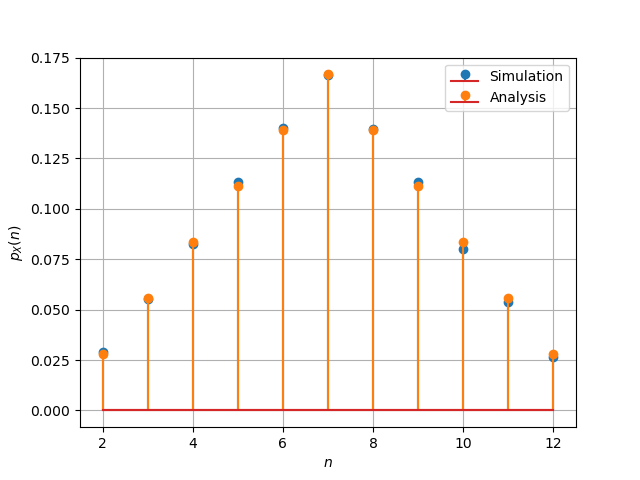
\includegraphics[width=0.75\linewidth]{figs/dice_pmf.png}
    \caption{PMF of the sum of two fair dice: Simulation vs Analysis}
    \label{fig:EE26BTECH11229-11}
\end{figure}
\item If a person completes a work in $t$ days, the rate of work is $\frac{1}{t}$ of the work per day. The rates of persons working together add up,
\begin{align}
	\frac{1}{t} = \frac{1}{t_1} + \frac{1}{t_2}
	\label{eq:EE26BTECH11229-work}
\end{align}
\item The angle of depression of an object $\vec{C}$ from a point $\vec{T}$ is equal to the angle of elevation of $\vec{T}$ from $\vec{C}$ (alternate angles). If $\vec{O}$ is the foot of the perpendicular from $\vec{T}$ to the ground, this angle $\theta$ is the angle between $\vec{T}-\vec{C}$ and $\vec{O}-\vec{C}$. From \eqref{eq:EE26BTECH11229-angle-vec},
\begin{align}
	\cos\theta = \frac{\brak{\vec{T}-\vec{C}}^{\top}\brak{\vec{O}-\vec{C}}}{\norm{\vec{T}-\vec{C}}\norm{\vec{O}-\vec{C}}}
	\label{eq:EE26BTECH11229-depression}
\end{align}
\item The points on the internal bisector of the angle at a vertex $\vec{A}$, with adjacent vertices $\vec{B}$ and $\vec{D}$, are
\begin{align}
	\vec{x} = \vec{A} + t\brak{\frac{\vec{B}-\vec{A}}{\norm{\vec{B}-\vec{A}}} + \frac{\vec{D}-\vec{A}}{\norm{\vec{D}-\vec{A}}}}, \quad t \in \mathbb{R}
	\label{eq:EE26BTECH11229-angle-bisector}
\end{align}
\solution
The two terms in the bracket are unit vectors along the sides $\vec{A}\vec{B}$ and $\vec{A}\vec{D}$. Their sum is the diagonal of a rhombus, which bisects the angle between them, yielding \eqref{eq:EE26BTECH11229-angle-bisector}.
\item The distance of a point $\vec{O}$ from the line passing through $\vec{P}$ with normal vector $\vec{n}$ is
\begin{align}
	d = \frac{\abs{\vec{n}^{\top}\brak{\vec{O}-\vec{P}}}}{\norm{\vec{n}}}
	\label{eq:EE26BTECH11229-dist-line}
\end{align}
\solution
The distance is the length of the projection of $\vec{O}-\vec{P}$ on $\vec{n}$, yielding \eqref{eq:EE26BTECH11229-dist-line}.
\end{enumerate}
